\documentclass[../thesis.tex]{subfiles}

\providecommand{\zcut}{z_\mathrm{{cut}}}


\setlength{\parskip}{0pt}
%%
%% End Preamble
%%
%% The fun begins:
\begin{document}
	Fixed-order calculations like that of Chapter \ref{chap:leading order} are nice because of their exactness, but because of the relatively large value the strong coupling, $\alpha_s \sim 0.1$, one must go to fairly high orders to obtain precise results. At low orders, the calculations are relatively straightforward, but this quickly ceases to be the case, as the number of event topologies that one must consider increases factorially with the order of $\alpha_s$. Moreover, and more pressingly, when we compute an exclusive cross section like $\sigma(e^+ e^- \to \text{hemisphere jets})$ in the presence of mMDT grooming, external energy scales are imposed. This is problematic for QCD, which is an intrinsically scale-invariant theory, and our punishment is the appearance of logarithms of scales which might grow large in particular limits, like the limit $\rho \sim \zcut \ll 1$ which we are considering \cite{larkoski_elementary_2019-1}. All this is to say that, while fixed-order calculations are nice for developing intuition for a physical quantity, they have limitations which become quite severe in the regime in which we are interested.

	We would therefore like to develop an alternative framework for calculating the distribution of heavy hemisphere mass. The strategy we will settle on is try to develop an \textbf{all-orders calculation} of the distribution. This result will take into account contributions at every order of $\alpha_s$, and provide a mathematical structure for producing arbitrarily accurate predictions, given sufficiently precise inputs. We will get there via the process of \textbf{resummation}, which will be discussed in Sec.~\ref{all-sec:resummation} (and, indeed, will occupy most of Chapter \ref{chap:all orders}). In order to prepare for that, we must first lay some groundwork.

	The first step on the path to an all-orders calculation is to derive a factorization formula for the heavy hemisphere mass cross section, the goal being to split the cross section into terms which each depend only on a single energy scale. The basic process for doing so is laid out in technical detail in Ref.~\cite{becher_introduction_2015-1}, and an example of a similar flavor to our calculation is provided by Frye et al.\ in Ref.~\cite{frye_factorization_2016}.\footnote{Indeed, the calculation of Frye et al.\ is a more general factorization of mass-like variables in groomed jets. Setting $\alpha = 2, \beta = 0$ for their two-point energy correlation function $e_2^{(\alpha)}$ under soft drop grooming with angular exponent $\beta$ yields the mMDT-groomed jet mass $\rho$. Their factorization is valid in the limit $\rho \ll \zcut \ll 1$, whereas we are interested in the limit $\rho \sim \zcut \ll 1$.} Once the cross section has been split into functions of single energy scales, the process of resummation can begin. 

	There are two primary steps in developing a factorization formula:
	\begin{enumerate}
		\item \textbf{Power counting}: this involves determining the possible radiative modes of an event and their dominant momentum scales. The term `power counting' refers to the fact that for some momentum scale $\lambda$, different radiative modes have momenta that scale as different powers of $\lambda$.

		\item \textbf{Factorization and refactorization}: Once the different radiative modes and energy scales are identified, we can use the framework of SCET to split the cross section into a convolution of terms describing different radiative modes. These terms themselves must then be split (refactored) into convolutions of terms, each of which depends, to leading order, only on a single energy scale.
	\end{enumerate}
	In this chapter, we will follow these steps to derive a factorization formula for the heavy hemisphere mass in the $\rho \sim \zcut \ll 1$ limit.

\section{Setup}
	One way to define the hemisphere mass is
	\begin{equation}
		\rho = \frac{1}{E_J^2} \sum_{i<j} 2p_i \cdot p_j
	\end{equation}
	with $E_J$ the jet energy and the sum ranging over all pairs of particles in the jet. Expanding out the dot product, we have
	\begin{equation}\label{factor-eq:jet mass z theta}
		\rho = \frac{2}{E_J^2} \sum_{i<j} \qty(E_i E_j - \vb{p}_i \cdot \vb{p}_j) = \frac{2}{E_J^2} \sum_{i<j} E_i E_j \qty(1 - \cos\theta_{ij}) = \sum_{i<j}2z_i z_j \qty(1 - \cos\theta_{ij}).
	\end{equation}
	Here, $z_i$ and $z_j$ are the relative energy fractions of each particle and $\theta_{ij}$ is the angle between particles $i$ and $j$.

	Throughout the following discussion, with $n^\mu$ the jet direction and $\bar n^\mu$ the direction opposite the jet, we will describe momenta in light-cone coordinates
	\begin{equation}
		p^\mu = \qty(p^-, p^+, p_\perp)
	\end{equation}
	with
	\begin{align}
		p^- &= \bar n \cdot p & p^+ &= n \cdot p
	\end{align}
	and $p_\perp$ the components of momentum transverse to $n$. In these coordinates, the energy fraction with respect to total energy $E_J = Q$ is
	\begin{equation}\label{factor-eq:z light cone coordinates}
		z = \frac{p^+ + p^-}{2Q}
	\end{equation}
	and, in the collinear limit, the angle to the jet axis is $\theta \approx p_\perp / p^0$ \cite{frye_factorization_2016}.
	
	In an $e^+ e^- \to \text{jets}$ event, there are two types of emission: resolved and unresolved. The essential difference is that a resolved emission is one which manifests itself as a jet at a particular scale of observation, while an unresolved emission does not. The presence of unresolved emissions can, however, perturb observable values of a resolved emission.

	Suppose now that we have applied an mMDT groomer with energy fraction cutoff $\zcut$. Then every \textit{resolved} emission must satisfy
	\begin{equation}
		z_i > \zcut,
	\end{equation}
	while other emissions with $z_i < \zcut$ can only pass the groomer if they are at a sufficiently small angle to a resolved emission.

\section{Power counting}
\subsection{Resolved soft emission}
	The primary emission contributing to the jet mass in the limit $\rho \sim \zcut \ll 1$ is a gluon emission $z_i$ sensitive to both $\rho$ and $\zcut$. In the presence of a hard quark with $z_q \sim 1$, the leading contributions to the jet mass of Eq.~\ref{factor-eq:jet mass z theta} are
	\begin{equation}
		\rho \approx \sum_i 2z_i \qty(1 - \cos\theta_i)
	\end{equation}
	where $\theta_i$ is the angle of emission $i$ from the quark. Considering the case with only one such emission,\footnote{This is the first-order approximation. One can consider additional resolved gluons to obtain a more precise result, but that is beyond what we require here.} we have
	\begin{equation}
		\rho \approx z_i \qty(1 - \cos\theta_i).
	\end{equation} 
	But since $z_i \sim \zcut$ and $\rho \sim \zcut$, this means that
	\begin{equation}
		\rho \approx \rho \qty(1 - \cos\theta_i),
	\end{equation}
	so
	\begin{equation}
		\cos\theta_i \ll 1.
	\end{equation}
	This means that
	\begin{equation}
		\theta_i \sim \frac{\pi}{2}.
	\end{equation}
	Since this emission is sensitive to $\zcut \ll 1$, we can also conclude that $z_i \ll 1$. Thus, we see that the leading contribution to the cusp region comes from a \textbf{resolved soft, wide-angle} gluon. Its momentum scales like
	\begin{equation}
		p_R \sim \zcut Q \qty(1, 1, 1).
	\end{equation}
	For future reference, let this gluon have energy fraction $z_R$ and angle $\theta_R$ from the quark axis.

	When this soft emission is resolved, it manifests itself in a detector as a jet. We therefore also need to consider the arbitrary \textbf{collinear} emissions off of the resolved gluon. If this radiation were hard, it would be resolved instead, so it must be soft like the resolved quark. The radiation collinear to the resolved gluon is therefore also sensitive to the scale $\zcut$.

\subsection{Ungroomed extra-soft unresolved radiation}
	\begin{figure}
	\begin{centering}
		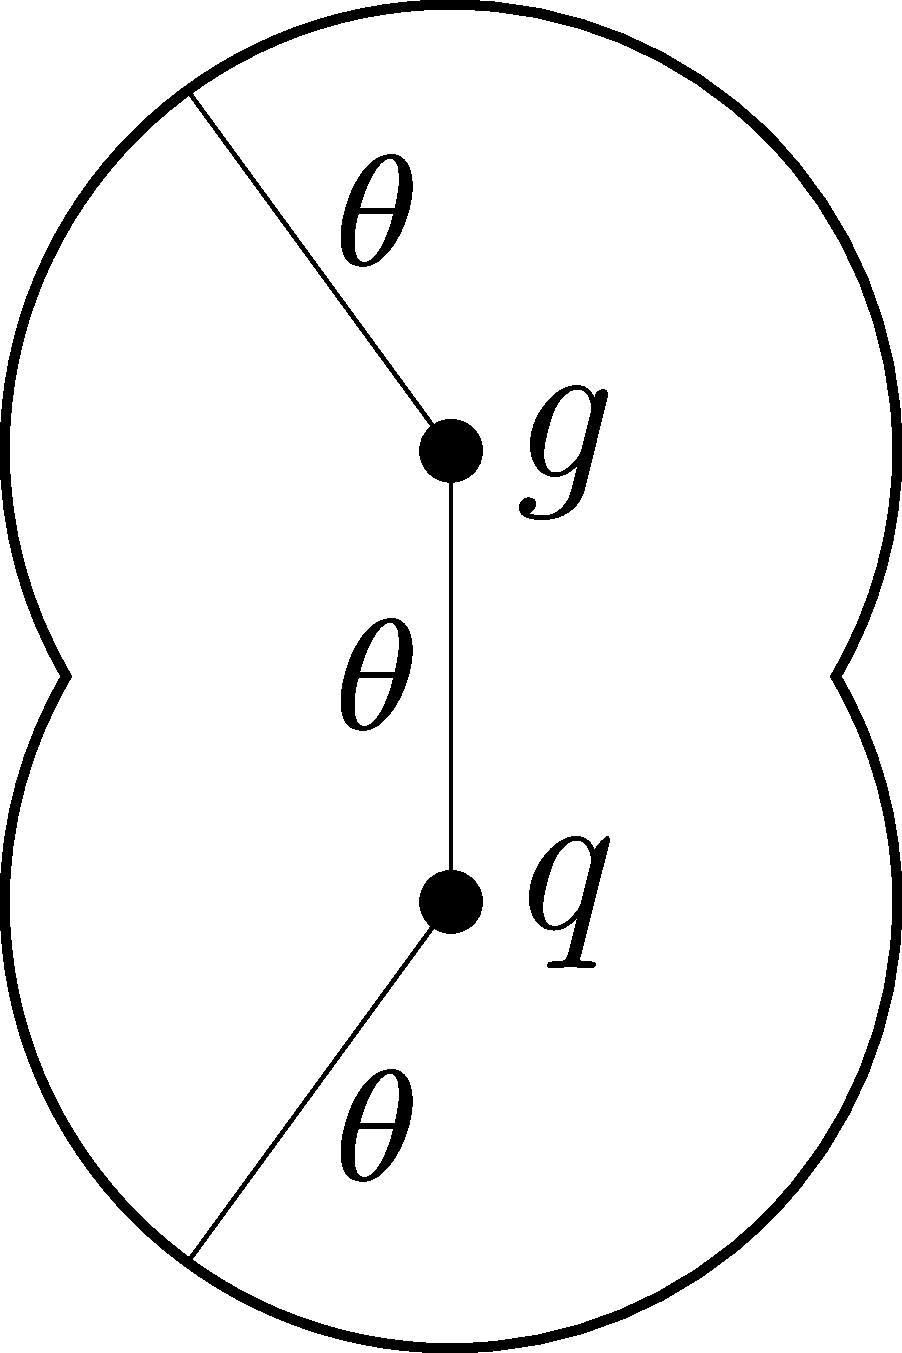
\includegraphics[width=0.2\columnwidth]{figures/head_on_schematic.pdf}
		\caption{\label{fig:head-on schematic}Head-on schematic of a quark jet $q$ and a resolved gluon $g$. If the angle between the quark and the gluon is $\theta$ and the gluon (plus all lower-scale unresolved radiation) passes the groomer, then the mMDT groomer will accept all radiation within an angle $\theta$ of both the quark and the resolved gluon.}
	\end{centering}
	\end{figure}
	Unresolved soft emissions can also contribute to the jet mass if they are sufficiently close to the resolved emission or the quark. Suppose there is another emission $i$ with energy fraction $z_i$ at angle $\theta_i$ from the jet axis and angle $\theta_{iR}$ from the resolved gluon. If $\theta_i < \theta_R$ or $\theta_{iR} < \theta_R$, a situation displayed in Fig.~\ref{fig:head-on schematic}, then emission $i$ will pass the groomer.

	What does this mean for the hemisphere mass? Well, first notice that since $\theta_R \sim \pi/2$, most soft radiation in the hemisphere passes this cut. The effect of these extra-soft emissions, which have $z_i \ll z_R$, is to perturb the mass of the resolved emission, so that the hemisphere mass is approximately
	\begin{equation}
		\rho \sim z_R + \sum_i z_i(1 - \cos\theta_i).
	\end{equation}
	The dominant contributions come again from the wide-angle emissions with $1 - \cos\theta_i \sim 1$; these must evidently have an energy scale set by
	\begin{equation}
		\rho - z_R \sim \sum_i z_i.
	\end{equation}
	Hence, since $z_R \sim \zcut$, the unresolved extra-soft emissions must scale as
	\begin{equation}
		p_{S_R} \sim \qty(\rho - \zcut)Q(1, 1, 1).
	\end{equation}

\subsection{Quark-collinear radiation}\label{sec:collinear radiation}
	We might also consider radiation collinear to a quark-jet axis with angle $\theta_i \ll 1$. This radiation has $p^- \gg p^+$, which means from Eq.~\ref{factor-eq:z light cone coordinates} that
	\begin{equation}
		z \approx \frac{p^+}{2Q}.
	\end{equation}
	Then because the particle must satisfy
	\begin{equation}
		z_i \theta_i^2 \lesssim \rho,
	\end{equation}
	we find that \cite{frye_factorization_2016}
	\begin{equation}
		\rho \sim \frac{p^+}{Q}.
	\end{equation}

	If $z \sim 1$, we know that $z \gg \zcut$, so the momentum scales independently of $\zcut$. Hence, the scaling of these \textbf{collinear} modes is \cite{frye_factorization_2016}
	\begin{equation}
		p_c \sim Q \qty(1, \rho, \rho^{1/2}).
	\end{equation}
	In a hemisphere where the resolved emission stops the mMDT groomer, this is the only collinear radiation that contributes.

	If on the other hand $z \sim \zcut \ll 1$, the result is \textbf{collinear-soft} radiation with $p^- \sim z_i Q$ and $p^+ \sim \theta_i^2 z_i Q$. From \cite{frye_factorization_2016}, these momenta scale like
	\begin{equation}
		p_{cs} \sim \zcut Q \qty(1, \frac{\rho}{\zcut}, \qty(\frac{\rho}{\zcut})^{1/2})
	\end{equation}
	and depend on the single energy scale $\sqrt{\rho\,\zcut}$. This scale matters in the hemisphere which does not contain the resolved soft gluon.


\section{Factorization}
	With the powers now counted, we are ready to derive a factorization formula describing the hemisphere mass distribution in the limit $\rho \sim \zcut \ll 1$. First, we should note that it is most straightforward to compute the double differential cross section in the masses of the individual hemispheres, then integrate over them to get the heavy hemisphere mass \cite{chien_resummation_2010}:
	\begin{equation}\label{factor-eq:heavy hemisphere cross section}
		\frac{d\sigma}{d\rho} = \int \frac{d^2\sigma}{d\rho_1d\rho_2}\qty[\delta(\rho - \rho_1)\Theta(\rho_1 - \rho_2) + \delta(\rho - \rho_2)\Theta(\rho_2 - \rho_1)].
	\end{equation}
	The integral simply breaks up the two cases $\rho_1 > \rho_2$ and $\rho_2 > \rho_1$ and assigns the correct value of $\rho$ in each case.

	Now, in the limit $\rho_1, \rho_2 \ll 1$, we can apply the technology of SCET to factorize the double-differential cross section into a product of hard, soft, and jet contributions \cite{frye_factorization_2016,ellis_jet_2010}. The basic form separates the event into a hard contribution, soft radiation, and two jets:
	\begin{equation}
		\frac{d^2\sigma}{d\rho_1 d\rho_2} = H(Q^2) \otimes S(\rho_1, \rho_2, \zcut) \otimes J_q(\rho_1) \otimes J_{\bar q}(\rho_2).
	\end{equation}
	The symbol $\otimes$ represents convolution. Here, $Q^2$ is the squared center-of-mass energy of the collision. $H(Q^2)$ is hard function representing the cross section of $e^+ e^- \to q\bar{q}$ events, $S(\rho_1, \rho_2, \zcut)$ is the function representing soft contributions (which are sensitive to $\zcut$), and $J_i(\rho)$ is a function describing the production of a jet off of particle $i$ (where $i$ is a quark $q$ or antiquark $\bar q$).

	As this factorization currently stands, several terms depend on multiple scales and must be refactored. In the limit $\rho \sim \zcut \ll 1$ after mMDT grooming, the soft function consists of global soft emissions which contribute only to the normalization; a resolved soft, wide-angle emission generated by a fixed-order function; radiation in a jet collinear to the resolved emission; and other soft, wide-angle radiation which passes the groomer due to the presence of the resolved emission. The first two depend only on the scale $\zcut$ and can be combined into one function. Therefore, we can write
	\begin{equation}
	\begin{aligned}
		\frac{d^2\sigma}{d\rho_1 d\rho_2} = H(Q^2) \times R(\rho_1, \rho_2, \zcut) \times S_R(\rho - \zcut) &\otimes J_{c, g}(\rho, \zcut)\\
			& \otimes J_{c, q}(\rho_1, \zcut) \otimes J_{c, \bar q}(\rho_2, \zcut).
	\end{aligned}
	\end{equation}
	The variable $\rho$ is used as a stand-in for either $\rho_1$ or $\rho_2$. Here, $R(\rho_1, \rho_2, \zcut)$ describes the resolved emission as well as other soft wide-angle radiation (from which the resolved emission emerged), while $S_R(\rho - \zcut)$ describes radiation which passes the groomer in the presence of the resolved emission. We have also introduced a jet function corresponding to the resolved gluon and re-written all of the jet functions as $J_{c, i}(\rho, \zcut)$ (where $i$ is either a quark $q$, an antiquark $\bar q$, or a gluon $g$) to make explicit their possible dependence on multiple scales.

	Now, as we established in Sec.~\ref{sec:collinear radiation}, radiation collinear to a quark jet with energy fraction of order 1 depends only on $\rho$, and radiation with energy fraction much less than 1 depends on the scale $\sqrt{\rho\,\zcut}$. However, this soft-collinear radiation only matters in the absence of a resolved gluon emission (which stops the mMDT groomer), in which case the jet function factorizes as
	\begin{equation}
		J_{c, \bar q}(\rho, \zcut) = J_{\bar q}(\rho) \otimes S_C(\sqrt{\rho\,\zcut}),
	\end{equation}
	where $J_{\bar q}(\rho)$ describes the antiquark jet function and $S_C(\sqrt{\rho\,\zcut})$ describes the soft-collinear radiation. The result is that we must treat each hemisphere separately, since one contains the resolved emission and the other does not. Therefore, if we assume, without loss of generality, that $\rho_1 > \rho_2$ (and introduce a factor of 2 to compensate for the restriction), the cross section becomes
	\begin{equation}\label{factor-eq:factorization formula}
	\boxed{
	\begin{aligned}
		\frac{d^2\sigma}{d\rho_1 d\rho_2} = 2 H(Q^2) \times R(\rho_1, \rho_2, \zcut) &\times S_R(\rho - \zcut) \otimes J_{g}(\zcut)\\
			& \otimes J_{q}(\rho_1) \otimes \qty[J_{\bar q}(\rho_2) \otimes S_C(\sqrt{\rho_2\,\zcut})].
	\end{aligned}
	}
	\end{equation}
	The functions $J_g,$ $J_q$, and $J_{\bar q}$ describe the gluon, quark, and antiquark jets, respectively. 

	This is our final factorization formula for the double differential cross section in each hemisphere mass. The distribution of the heavy hemisphere mass then given by Eq.~\ref{factor-eq:heavy hemisphere cross section}. We are now ready to proceed with resummation.

% \ifstandalone
% \bibliographystyle{../bsts/JHEP} 
% \bibliography{../jet_substructure}
% \fi
\end{document}
